\documentclass[11pt,a4paper]{article}

% Packages
\usepackage[utf8]{inputenc}
\usepackage[spanish, es-tabla]{babel}
\usepackage{parskip}
\usepackage{enumerate}
\usepackage{graphicx}
\usepackage{subfigure}
\usepackage{float}
\usepackage{amsmath}


\usepackage[bookmarks=true,
					 bookmarksnumbered=false,
					 bookmarksopen=false,
					 colorlinks=true,
					 allcolors=blue,
					 urlcolor=blue]{hyperref}

\usepackage[ruled]{algorithm2e}
\SetKwInOut{Parameter}{parameter}

\usepackage{array}
\newcolumntype{N}{>{\centering\arraybackslash}m{0.5cm}}
\newcolumntype{M}{>{\centering\arraybackslash}m{1cm}}

\usepackage[left=2cm, right=2cm, top=2cm, bottom=2cm]{geometry}

\begin{document}\pagenumbering{arabic}
\begin{titlepage}
\centering
\includegraphics[width=0.15\textwidth]{/Users/pedrors/Desktop/DGIIM/Latex/UGR}\par\vspace{1cm}
{\scshape\LARGE Universidad de Granada \par}
\vspace{1cm}
{\Huge\bfseries Práctica Final\par}
{\Large\bfseries Metaheurística basada en cargas eléctricas
\par}
\vspace{1.5cm}
{\huge\bfseries Metaheurísticas\par}
{\large\bfseries Grupo 2 (Lunes)\par}
\vspace{2cm}
{\Large\itshape Pedro Ramos Suárez\par}
{\large\itshape 76591270M\par}
{\large\itshape pedrors@correo.ugr.es\par}
\vfill
Doble Grado de Ingeniería Informática y Matemáticas
\vfill
{\large \today \par}
\author{A}
\end{titlepage}

\tableofcontents
\newpage
\section{Problema de Aprendizaje de Pesos en Características} \label{sect:APC}

\subsection{Descripción del problema}

El problema consiste en optimizar el rendimiento de un clasificador basado en el vecino más cercano a partir de la inclusión de pesos asociados a las características del problema.

El clasificador utilizado es el 1-NN (1 vecino más cercano), el cuál consiste en asignar a cada nuevo la misma etiqueta que a su vecino más cercano. Para ello, utilizamos la distancia euclídea modificada por unos pesos asociados a cada característica:
$$d(e_{1}, e_{2}) = (\sum_{i=1}^{n} w_{i} \cdot (e_{1}^{i} - e_{2}^{i})^{2})^{\frac{1}{2}}$$
donde $n$ es el número de características de los datos, y $W = (w_{1}, \dots, w_{n})$ el vector de números reales entre 0 y 1 que define el peso que pondera cada una de las características.

La variante que intentaremos optimizar será la agregación, que combina tanto la precisión como la complejidad del clasificador, definida como:
\begin{equation} \label{eq:objetivo}
\text{Agregación}(W) = \alpha \cdot \text{Tasa\_clas}(W) + (1 - \alpha) \cdot \text{Tasa\_red}(W)
\end{equation}
donde:
\begin{equation} \label{eq:clas}
\text{Tasa\_clas} = 100 \cdot \frac{\text{nº de instancias bien clasificadas en T}}{\text{nº de instancias en T}}
\end{equation}
\begin{equation} \label{eq:red}
\text{Tasa\_red} = 100 \cdot \frac{\text{nº de valores } w_{i} < 0.1}{\text{nº de características}}
\end{equation}

siendo $T$ el conjunto de datos sobre los que se evalúa el clasificador, y $\alpha$ es un número real entre 0 y 1 que pondera la importancia entre acierto y la reducción de la solución.

\subsection{Datos utilizados}

Los datos utilizados serán:
\begin{enumerate}
\item \textbf{Ionosphere}: Conjunto de datos de radar, formado por 351 ejemplos con 34 características clasificados en dos clases.
\item \textbf{Parkinsons}: Conjunto de datos orientados a distinguir entre la presencia y ausencia de la enfermedad de Parkinson en una serie de pacientes, formado por 195 ejemplos con 22 características clasificados en dos clases.
\item \textbf{Spectf-heart}: Conjunto de datos de detección de enfermedades cardíacas a partir de imágenes médicas de termografía computerizada del corazón, formada por 349 ejemplos con 44 características clasificados en dos clases.
\end{enumerate}

\newpage
\section{Descripción de la metaheurística basada en cargas}

\subsection{Idea general}

Para esta práctica vamos a desarrollar una metaheurística propia. Inicialmente, mi idea era bastante simple: partimos de un conjunto inicial aleatorio de soluciones, y estas atraerán a las demás si son mejores, o las rechazaran si son peores. Esto me dio la idea de basarme en un sistema real: las cargas eléctricas.

Una carga eléctrica atrae a otra si sus cargas son de signo opuesto, y la repele si las cargas son del mismo signo. Además, estas fuerzas son inversamente proporcional a la distancia, es decir, si dos cargas están más cerca, la fuerza será mayor. La fórmula de la fuerza de atracción o repulsión entre cargas es:
$$F = k \frac{q_{1}q_{2}}{r^{2}}$$
donde $F$ es la fuerza, $k$ la constante de Coulomb ($8.987 \times 10^{9} N \cdot m^{2} / C^{2}$), $q_{i}$ es la magnitud de las cargas y $r$ es la distancia entre ellas.

\subsection{Implementación de la metaheurística}

En nuestro caso, como las soluciones no tienen signo, haremos que actúen como si tuvieran signo opuesto si son mejores o como si tuvieran el mismo signo si son peores. Además, para hacer la metaheurística más eficiente, en lugar de que todas las soluciones atraigan o repelan a las demás, podemos hacer que únicamente la mejor solución atraiga a las demás, y la peor repela a las demás.

Sin embargo, esto nos da un problema. Si suponemos que la mejor solución ha encontrado el máximo o mínimo que buscamos, la peor solución le empujará, obteniendo una solución peor. Debido a ello, la peor solución repelerá a todas menos a la mejor.

Otro problema que tenemos es si dos soluciones son iguales. En este caso, la distancia será 0, por lo que al dividir entre 0 tendremos un error. Para solucionarlo, utilizaremos:
$$F = k q_{1}q_{2} (1 - r^{2})$$
De esta forma sigue siendo inversamente proporcional a las distancias, pero no tenemos que dividir entre 0 en ningún caso. Además, la constate sólo tiene sentido en el caso de cargas eléctricas, por lo que la eliminamos. Así, finalmente nos queda:
$$F = q_{1}q_{2} (1 - r^{2})$$

Para aumentar eficiencia, en vez de calcular la distancia euclídea entre dos soluciones, utilizaremos la distancia en fitness que, como ya tenemos calculados los fitness para saber cuál es la mejor y cuál es la peor solución, no nos llevará ningún tiempo.

Por último, tras cada iteración, para aumentar la exploración, sustituimos una solución aleatoria que no sea la mejor por una nueva solución aleatoria.

Con todo esto, el algoritmo queda de la forma: \\
\begin{algorithm}[H]
	\caption{{\sc Charges} metaheurística basada en cargas eléctricas.}
	Iniciar una población aleatoria de soluciones. \\
	\While{No se cumpla la condición de parada}{
		Buscamos la mejor solución. \\
		Buscamos la peor solución. \\
		Movemos todas las soluciones por la fuerza de atracción hacia la mejor solución. \\
		Movemos todas menos la mejor solución por la fuerza de repulsión en dirección opuesta a la peor solución. \\
		Sustituimos una solución que no sea la mejor por una aleatoria.
	}
	\Return{La mejor solución.}
\end{algorithm}

\newpage
\section{Implementación al Problema de Aprendizaje en Pesos en Características}

Adaptamos la metaheurística explicada en la sección anterior al problema desarrollado durante las prácticas previas, el Problema de Aprendizaje en Pesos en Características, explicado en la sección \eqref{sect:APC}.

El código queda de la forma: \\
\begin{footnotesize}
\begin{algorithm}[H]
	\caption{{\sc Charges} metaheurística basada en cargas eléctricas.}
	\KwIn{La matriz de características $x$.}
	\KwIn{El vector de etiquetas $y$.}
	\KwIn{El número de cromosomas $chromosomes$.}
	\KwIn{El número máximo de evaluaciones $evalutations$.}
	\KwOut{El vector de pesos obtenidos de la metaheurística.}
	
	$solutions \gets \{\}$ \;
	$fitness \gets \{\}$ \;
	$eval \gets 0$ \;
	\For{$chromosome$ \textbf{in} $\{0, \dots, chromosomes\}$}{
		$solutions \gets$ Solución inicial aleatoria \;
		$fitness \gets \operatorname{agregation}(solutions[i])$ \;
		$eval \gets eval + 1$ \;
	}
	
	\While{$eval < evaluations$}{
		$bestSolution \gets$ La posición de la mejor solución en $solutions$ \;
		$bestFitness \gets fitness[bestSolution]$ \;
		$worstSolution \gets$ La posición de la peor solución en $solutions$ \;
		$worstFitness \gets fitness[worstSolution]$ \;
		
		\For{$i$ \textbf{in} $\{0, \dots, chromosomes\}$}{
			\If{$i != bestSolution$}{
				$pullForce \gets fitness[i] \cdot fitness[bestSolution] \cdot (1 - (bestFitness - fitness[i])^{2})$ \;
				$pushForce \gets fitness[i] \cdot fitness[worstSolution] \cdot (1 - (worstFitness - fitness[i])^{2})$ \;
				
				$solutions[i] \gets (solutions[bestSolution] - solutions[i]) \cdot pullForce$ \;
				\If{$i != worstSolution$}{
					$solutions[i] \gets (solutions[i] - solutions[worstSolution]) \cdot pushForce$ \;
				}
				$fitness[i] \gets \operatorname{agregation}(solutions[i])$ \;
				$eval \gets eval + 1$ \;
			}
		}
		$soltions[bestSolution] \gets \operatorname{localSearch}(bestSolution)$ \;
		$fitness[i] \gets \operatorname{agregation}(solutions[i])$ \;
		$eval \gets eval + 1$ \;
		
		$rand \gets$ Número aleatorio en $\{0, \dots, chromosomes\}$ distinto de $bestSolution$ \;
		$solutions[rand] \gets$ Solución aleatoria.
	}
	
	\Return{$solutions[bestSolution]$}
\end{algorithm}
\end{footnotesize}

Utilizaremos 30 cromosomas (o soluciones), y un máximo de 15000 evaluaciones. Como datos utilizaremos los leídos de las distintas bases de datos, separando en 5 conjuntos distintos de entrenamiento y test (de forma que cada dato actúa una vez como test y cuatro veces como entrenamiento).

\subsection{Resultados obtenidos}

Los resultados que obtenemos de aplicar el algoritmo \emph{charges} al problema de Aprendizaje en Pesos son:

\begin{table}[H] \label{tab:charges}
\centering \tiny
\begin{tabular}{ M | c  c  c  c | c  c  c  c | c  c  c  c |}
\cline{2-13}
 & \multicolumn{4}{c|}{Ionosphere} & \multicolumn{4}{c|}{Parkinsons} & \multicolumn{4}{c|}{Spectf-heart} \\ \cline{2-13}
\multicolumn{1}{c|}{ } & \%\_clas & \%\_red & Agr. & T & \%\_clas & \%\_red & Agr. & T & \%\_clas & \%\_red & Agr. & T \\ \hline
\multicolumn{1}{|c|}{Partición 1} & 88.73 & 94.12 & 91.43 & 246.93 & 89.74 & 86.36 & 88.05 & 76.55 & 87.14 & 93.18 & 90.16 & 264.32 \\ \hline
\multicolumn{1}{|c|}{Partición 2} & 95.71 & 91.18 & 93.45 & 254.15 & 89.74 & 90.91 & 90.33 & 75.73 & 87.14 & 93.18 & 90.16 & 263.89 \\ \hline
\multicolumn{1}{|c|}{Partición 3} & 82.86 & 94.12 & 88.49 & 254.18 & 94.87 & 81.82 & 88.34 & 76.11 & 81.43 & 93.18 & 87.31 & 263.06 \\ \hline
\multicolumn{1}{|c|}{Partición 4} & 90.00 & 91.18 & 90.59 & 253.42 & 94.87 & 90.91 & 92.89 & 76.22 & 80.00 & 93.18 & 86.59 & 265.72 \\ \hline
\multicolumn{1}{|c|}{Partición 5} & 91.43 & 91.18 & 91.30 & 256.59 & 92.31 & 90.91 & 91.61 & 75.63 & 84.06 & 93.18 & 88.62 & 264.24 \\ \hline \hline
\multicolumn{1}{|c|}{Media} & 89.75 & 92.35 & 91.05 & 253.05 & 92.31 & 88.18 & 90.24 & 76.05 & 83.95 & 93.18 & 88.57 & 264.24 \\ \hline
\end{tabular}
\caption{Tabla con los resultados obtenidos con el algoritmo charges.}
\end{table}

\newpage
\section{Hibridación con búsqueda local}

Al igual que hicimos con los algoritmos genéticos, vamos a probar a añadir una búsqueda local a ciertas soluciones tras un cierto número de iteraciones. Esta vez se lo aplicaremos de la misma forma que la que nos solía dar mejores resultados en el algoritmo memético, que era a un 10 \% aleatorio de la población.

Inicialmente, intenté mantener los mismos parámetros que usamos con el algoritmo memético: 10 cromosomas, y aplicamos la búsqueda local cada 10 iteraciones. Sin embargo, esto producía resultados mucho peores a los esperados.

Tras probar varias ejecuciones con distinto número de cromosomas y de iteraciones entre cada búsqueda local, los mejores resultados obtenidos fueron con 30 cromosomas y aplicando búsqueda local cada 30 iteraciones.

Esto nos demuestra como, debido a que obtenemos mejores soluciones haciendo que las soluciones actuales interactúen entre ellas, es importante un número alto de cromosomas, y debido a que tomar un número tan alto de cromosomas provoca que muchas evaluaciones sean durante la búsqueda local, también es importante aumentar el número de iteraciones entre cada búsqueda local.

\subsection{Resultados obtenidos}

Los resultados obtenidos con 30 cromosomas y aplicando la búsqueda local cada 30 iteraciones son:

\begin{table}[H] \label{tab:chargesMemetic}
\centering \tiny
\begin{tabular}{ M | c  c  c  c | c  c  c  c | c  c  c  c |}
\cline{2-13}
 & \multicolumn{4}{c|}{Ionosphere} & \multicolumn{4}{c|}{Parkinsons} & \multicolumn{4}{c|}{Spectf-heart} \\ \cline{2-13}
\multicolumn{1}{c|}{ } & \%\_clas & \%\_red & Agr. & T & \%\_clas & \%\_red & Agr. & T & \%\_clas & \%\_red & Agr. & T \\ \hline
\multicolumn{1}{|c|}{Partición 1} & 92.96 & 91.18 & 92.07 & 259.76 & 76.92 & 90.91 & 83.92 & 77.93 & 85.71 & 93.18 & 89.45 & 271.79 \\ \hline
\multicolumn{1}{|c|}{Partición 2} & 94.29 & 91.18 & 92.73 & 259.84 & 92.31 & 90.91 & 91.61 & 77.85 & 90.00 & 90.91 & 90.45 & 270.77 \\ \hline
\multicolumn{1}{|c|}{Partición 3} & 84.29 & 94.12 & 89.20 & 264.68 & 82.05 & 90.91 & 86.48 & 78.18 & 82.86 & 93.18 & 88.02 & 270.81 \\ \hline
\multicolumn{1}{|c|}{Partición 4} & 94.29 & 91.18 & 92.73 & 260.56 & 97.44 & 81.82 & 89.63 & 78.33 & 88.57 & 90.91 & 89.74 & 270.54 \\ \hline
\multicolumn{1}{|c|}{Partición 5} & 87.14 & 94.12 & 90.63 & 260.44 & 97.44 & 81.82 & 89.63 & 78.25 & 84.06 & 93.18 & 88.62 & 273.38 \\ \hline \hline
\multicolumn{1}{|c|}{Media} & 90.59 & 92.35 & 91.47 & 261.06 & 89.23 & 87.27 & 88.25 & 78.11 & 86.24 & 92.27 & 89.26 & 271.46 \\ \hline
\end{tabular}
\caption{Tabla con los resultados obtenidos con el algoritmo chargesMemetic.}
\end{table}

\newpage
\section{Intentos de mejora}

\subsection{Metaheurística con exploración del mejor entorno}

Un posible problema que podemos ver en la metaheurística es que, como la fuerza es inversamente proporcional a la distancia, si está cerca de la mejor solución, la fuerza será mayor, lo cuál provoca que se aleje de esta mejor solución.

Para solucionar esto, una posible mejora es, tras cada iteración, aplicar una búsqueda local a la mejor solución y así explorar su entorno. Esto nos puede recordar al algoritmo memético, sin embargo, hay dos diferencias: únicamente aplicamos la búsqueda local a la mejor solución, y además, como la aplicamos cada iteración, el número de vecinos explorados en cada búsqueda local es menor.

\subsection{Resultados de la metaheurística con exploración del mejor entorno}

Los resultados obtenidos con \emph{chargesBl} son:

\begin{table}[H] \label{tab:chargesBl}
\centering \tiny
\begin{tabular}{ M | c  c  c  c | c  c  c  c | c  c  c  c |}
\cline{2-13}
 & \multicolumn{4}{c|}{Ionosphere} & \multicolumn{4}{c|}{Parkinsons} & \multicolumn{4}{c|}{Spectf-heart} \\ \cline{2-13}
\multicolumn{1}{c|}{ } & \%\_clas & \%\_red & Agr. & T & \%\_clas & \%\_red & Agr. & T & \%\_clas & \%\_red & Agr. & T \\ \hline
\multicolumn{1}{|c|}{Partición 1} & 91.55 & 91.18 & 91.36 & 260.79 & 97.44 & 81.82 & 89.63 & 76.64 & 88.57 & 90.91 & 89.74 & 264.45 \\ \hline
\multicolumn{1}{|c|}{Partición 2} & 88.57 & 94.12 & 91.34 & 259.63 & 94.87 & 90.91 & 92.89 & 76.37 & 85.71 & 93.18 & 89.45 & 265.04 \\ \hline
\multicolumn{1}{|c|}{Partición 3} & 92.86 & 91.18 & 92.02 & 256.07 & 87.18 & 81.82 & 84.50 & 76.50 & 85.71 & 93.18 & 89.45 & 264.22 \\ \hline
\multicolumn{1}{|c|}{Partición 4} & 82.86 & 91.18 & 87.02 & 255.91 & 84.62 & 90.91 & 87.76 & 76.34 & 87.14 & 88.64 & 87.89 & 267.07 \\ \hline
\multicolumn{1}{|c|}{Partición 5} & 90.00 & 91.18 & 90.59 & 257.23 & 97.44 & 90.91 & 94.17 & 76.32 & 91.30 & 90.91 & 91.11 & 267.00 \\ \hline \hline
\multicolumn{1}{|c|}{Media} & 89.17 & 91.76 & 90.47 & 257.93 & 92.31 & 87.27 & 89.79 & 76.43 & 87.69 & 91.36 & 89.53 & 265.56 \\ \hline
\end{tabular}
\caption{Tabla con los resultados obtenidos con el algoritmo chargesBl.}
\end{table}

\subsection{Metaheurística con distancia euclídea}

Cuando desarrollamos la metaheurística, decidimos tomar como distancia entre dos soluciones la diferencia en valor absoluto entre sus fitness, ya que es más eficiente que calcular la distancia euclídea. Esto nos hace preguntarnos, ¿qué pasaría si hubiesemos usado la distancia euclídea? Aunque el tiempo de ejecución fuese mayor, ¿obtendríamos mejores resultados?

Para eso desarrollamos una nueva versión modificada, que utilizará la distancia euclídea para el calculo de las fuerzas.

\subsection{Resultados de la metaheurística con la distancia euclídea}

Los resultados obtenidos con \emph{chargesEuclidean} son:

\begin{table}[H] \label{tab:chargesEuclidean}
\centering \tiny
\begin{tabular}{ M | c  c  c  c | c  c  c  c | c  c  c  c |}
\cline{2-13}
 & \multicolumn{4}{c|}{Ionosphere} & \multicolumn{4}{c|}{Parkinsons} & \multicolumn{4}{c|}{Spectf-heart} \\ \cline{2-13}
\multicolumn{1}{c|}{ } & \%\_clas & \%\_red & Agr. & T & \%\_clas & \%\_red & Agr. & T & \%\_clas & \%\_red & Agr. & T \\ \hline
\multicolumn{1}{|c|}{Partición 1} & 84.51 & 79.41 & 81.96 & 294.91 & 94.87 & 81.82 & 88.34 & 80.57 & 81.43 & 77.27 & 79.35 & 279.15 \\ \hline
\multicolumn{1}{|c|}{Partición 2} & 95.71 & 85.29 & 90.50 & 294.85 & 94.87 & 86.36 & 90.62 & 81.00 & 85.71 & 77.27 & 81.49 & 280.80 \\ \hline
\multicolumn{1}{|c|}{Partición 3} & 88.57 & 82.35 & 85.46 & 294.64 & 87.18 & 81.82 & 84.50 & 80.53 & 81.43 & 79.55 & 80.49 & 280.11 \\ \hline
\multicolumn{1}{|c|}{Partición 4} & 84.29 & 82.35 & 83.32 & 294.08 & 94.87 & 81.82 & 88.34 & 79.89 & 91.43 & 77.27 & 84.35 & 278.91 \\ \hline
\multicolumn{1}{|c|}{Partición 5} & 88.57 & 79.41 & 83.99 & 294.85 & 84.62 & 86.36 & 85.49 & 80.16 & 85.51 & 81.82 & 83.66 & 279.03 \\ \hline \hline
\multicolumn{1}{|c|}{Media} & 88.33 & 81.76 & 85.05 & 294.67 & 91.28 & 83.64 & 87.46 & 80.43 & 85.10 & 78.64 & 81.87 & 279.60 \\ \hline
\end{tabular}
\caption{Tabla con los resultados obtenidos con el algoritmo chargesEuclidean.}
\end{table}

\subsection{Metaheurística con exploración limitada}

La primera idea que se nos ocurre cuando pensamos en mejorar la metraheurística es mejorar las soluciones es obtenidas. Sin embargo, otra posible mejora es reducir el tiempo de ejecución

Esta idea se basa en la implementación que realizamos de la búsqueda local: si la metaheurística se queda ``atascada'', es decir, si realiza varias iteraciones sin encontrar ninguna mejora, se detiene.

Esto provocará que las soluciones sean iguales o peores, pero disminuirá el tiempo de ejecución, lo cuál puede ser interesante si la utilizamos en un sistema en tiempo real, para el cuál es importante asegurarse de que los tiempos no sean demasiados altos.

\subsection{Resultados de la metaheurística con exploración limitada}

Los resultados obtenidos con \emph{chargesMaxIter} son:

\begin{table}[H] \label{tab:chargesMaxIter}
\centering \tiny
\begin{tabular}{ M | c  c  c  c | c  c  c  c | c  c  c  c |}
\cline{2-13}
 & \multicolumn{4}{c|}{Ionosphere} & \multicolumn{4}{c|}{Parkinsons} & \multicolumn{4}{c|}{Spectf-heart} \\ \cline{2-13}
\multicolumn{1}{c|}{ } & \%\_clas & \%\_red & Agr. & T & \%\_clas & \%\_red & Agr. & T & \%\_clas & \%\_red & Agr. & T \\ \hline
\multicolumn{1}{|c|}{Partición 1} & 92.96 & 91.18 & 92.07 & 47.27 & 84.62 & 86.36 & 85.49 & 8.09 & 87.14 & 88.64 & 87.89 & 55.16 \\ \hline
\multicolumn{1}{|c|}{Partición 2} & 87.14 & 88.24 & 87.69 & 48.10 & 97.44 & 86.36 & 91.90 & 11.13 & 85.71 & 81.82 & 83.77 & 28.21 \\ \hline
\multicolumn{1}{|c|}{Partición 3} & 82.86 & 88.24 & 85.55 & 25.77 & 87.18 & 81.82 & 84.50 & 6.60 & 84.29 & 90.91 & 87.60 & 33.84 \\ \hline
\multicolumn{1}{|c|}{Partición 4} & 94.29 & 79.41 & 86.85 & 33.66 & 100.00 & 81.82 & 90.91 & 7.62 & 87.14 & 86.36 & 86.75 & 29.78 \\ \hline
\multicolumn{1}{|c|}{Partición 5} & 87.14 & 82.35 & 84.75 & 37.72 & 97.44 & 81.82 & 89.63 & 13.57 & 82.61 & 88.64 & 85.62 & 49.08 \\ \hline \hline
\multicolumn{1}{|c|}{Media} & 88.88 & 85.88 & 87.38 & 38.50 & 93.33 & 83.64 & 88.48 & 9.40 & 85.38 & 87.27 & 86.33 & 39.21 \\ \hline
\end{tabular}
\caption{Tabla con los resultados obtenidos con el algoritmo chargesMaxIter.}
\end{table}

\subsection{Metaheurística con reinicio}

La modificación con exploración limitada nos hace pensar otra posible modificación: en lugar de terminar la metahurística si se queda ``atascada'', podemos probar a reiniciar todas las soluciones actuales menos la mejor, es decir, cambiarlas por soluciones aleatorias.

De esta forma, cuando realicemos varias iteraciones sin mejora, crearemos muchas soluciones nuevas, lo cuál aumenta en gran medida la exploración.

\subsection{Resultados de la metaheurística con reinicio}

Los resultados obtenidos con \emph{chargesReset} son:

\begin{table}[H] \label{tab:chargesReset}
\centering \tiny
\begin{tabular}{ M | c  c  c  c | c  c  c  c | c  c  c  c |}
\cline{2-13}
 & \multicolumn{4}{c|}{Ionosphere} & \multicolumn{4}{c|}{Parkinsons} & \multicolumn{4}{c|}{Spectf-heart} \\ \cline{2-13}
\multicolumn{1}{c|}{ } & \%\_clas & \%\_red & Agr. & T & \%\_clas & \%\_red & Agr. & T & \%\_clas & \%\_red & Agr. & T \\ \hline
\multicolumn{1}{|c|}{Partición 1} & 94.37 & 91.18 & 92.77 & 251.44 & 89.74 & 90.91 & 90.33 & 75.05 & 84.29 & 93.18 & 88.73 & 259.29 \\ \hline
\multicolumn{1}{|c|}{Partición 2} & 91.43 & 88.24 & 89.83 & 251.38 & 89.74 & 90.91 & 90.33 & 75.16 & 90.00 & 93.18 & 91.59 & 259.31 \\ \hline
\multicolumn{1}{|c|}{Partición 3} & 90.00 & 91.18 & 90.59 & 263.81 & 92.31 & 90.91 & 91.61 & 75.28 & 90.00 & 90.91 & 90.45 & 259.61 \\ \hline
\multicolumn{1}{|c|}{Partición 4} & 90.00 & 91.18 & 90.59 & 253.77 & 89.74 & 90.91 & 90.33 & 75.16 & 84.29 & 90.91 & 87.60 & 258.56 \\ \hline
\multicolumn{1}{|c|}{Partición 5} & 94.29 & 91.18 & 92.73 & 251.47 & 87.18 & 90.91 & 89.04 & 75.28 & 89.86 & 93.18 & 91.52 & 258.89 \\ \hline \hline
\multicolumn{1}{|c|}{Media} & 92.02 & 90.59 & 91.30 & 254.37 & 89.74 & 90.91 & 90.33 & 75.19 & 87.69 & 92.27 & 89.98 & 259.13 \\ \hline
\end{tabular}
\caption{Tabla con los resultados obtenidos con el algoritmo chargesReset.}
\end{table}

\newpage
\section{Análisis de resultados}
Todos los resultados se han obtenido en un ordenador con las siguientes especificaciones:
\begin{itemize}
\item Sistema operativo: macOS Montery.
\item Procesador: 1,6 GHz Intel Core i5 de doble núcleo.
\item Memoria: 16 GB 2133 MHz LPDDR3.
\item Gráficos: Intel UHD Graphics 617 1536 MB.
\end{itemize}

El tiempo en las tablas es en segundos.

\subsection{Comparación de algoritmos}

\begin{table}[H] \label{tab:global}
\centering \tiny
\begin{tabular}{ M | c  c  c  c | c  c  c  c | c  c  c  c |}
\cline{2-13}
 & \multicolumn{4}{c|}{Ionosphere} & \multicolumn{4}{c|}{Parkinsons} & \multicolumn{4}{c|}{Spectf-heart} \\ \cline{2-13}
\multicolumn{1}{c|}{ } & \%\_clas & \%\_red & Agr. & T & \%\_clas & \%\_red & Agr. & T & \%\_clas & \%\_red & Agr. & T \\ \hline
\multicolumn{1}{|c|}{1-NN} & 86.89 & 0.00 & 43.45 & 0.02 & 96.41 & 0.00 & 48.21 & 0.00 & 86.25 & 0.00 & 43.12 & 0.02 \\ \hline
\multicolumn{1}{|c|}{RELIEF} & 72.60 & 2.94 & 37.77 & 0.02 & 96.41 & 0.00 & 48.21 & 0.01 & 83.68 & 0.00 & 41.84 & 0.02 \\ \hline
\multicolumn{1}{|c|}{BL} & 85.46 & 80.00 & 82.73 & 30.79 & 85.64 & 78.18 & 81.91 & 4.35 & 85.66 & 80.45 & 83.06 & 42.73 \\ \hline \hline

\multicolumn{1}{|c|}{ES} & 92.30 & 89.41 & 90.85 & 257.57 & 92.31 & 90.91 & 91.61 & 75.82 & 88.27 & 91.82 & 90.04 & 271.65 \\ \hline
\multicolumn{1}{|c|}{BMB} & 90.04 & 81.76 & 85.90 & 271.07 & 91.79 & 78.18 & 84.99 & 77.23 & 85.69 & 75.45 & 80.57 & 279.34 \\ \hline
\multicolumn{1}{|c|}{ILS} & 85.16 & 90.59 & 87.88 & 121.74 & 87.69 & 88.18 & 87.94 & 23.52 & 85.96 & 89.55 & 87.75 & 156.30 \\ \hline
\multicolumn{1}{|c|}{ILS-ES} & 86.03 & 91.76 & 88.90 & 174.25 & 89.74 & 90.91 & 90.33 & 49.95 & 84.23 & 91.36 & 87.80 & 174.90 \\ \hline \hline

\multicolumn{1}{|c|}{AGG-BLX} & 88.88 & 87.65 & 88.26 & 172.58 & 87.69 & 84.55 & 86.12 & 51.70 & 81.38 & 79.55 & 80.46 & 180.23 \\ \hline
\multicolumn{1}{|c|}{AGG-CA} & 86.60 & 87.65 & 87.12 & 172.90 & 89.74 & 89.09 & 89.42 & 51.00 & 84.24 & 82.73 & 83.48 & 180.16 \\ \hline
\multicolumn{1}{|c|}{AGE-BLX} & 88.32 & 81.76 & 85.04 & 172.36 & 90.26 & 74.55 & 82.40 & 51.22 & 83.66 & 78.18 & 80.92 & 178.96 \\ \hline
\multicolumn{1}{|c|}{AGE-CA} & 88.60 & 88.82 & 88.71 & 170.91 & 86.15 & 81.82 & 83.99 & 51.26 & 83.67 & 89.55 & 86.61 & 176.25 \\ \hline \hline

\multicolumn{1}{|c|}{AM-(10, 1.0)} & 86.61 & 87.06 & 86.84 & 174.83 & 91.28 & 87.27 & 89.28 & 51.91 & 85.66 & 74.55 & 80.11 & 182.01 \\ \hline
\multicolumn{1}{|c|}{AM-(10, 0.1)} & 87.18 & 91.18 & 89.18 & 164.92 & 89.74 & 89.09 & 89.42 & 49.45 & 85.39 & 87.73 & 86.56 & 175.95 \\ \hline
\multicolumn{1}{|c|}{AM-(10, 0.1mej)} & 87.47 & 70.00 & 78.73 & 169.39 & 84.62 & 87.27 & 85.94 & 49.45 & 83.40 & 50.00 & 66.70 & 180.71 \\ \hline \hline

\multicolumn{1}{|c|}{charges}  & 89.75 & 92.35 & 91.05 & 253.05 & 92.31 & 88.18 & 90.24 & 76.05 & 83.95 & 93.18 & 88.57 & 264.24 \\ \hline
\multicolumn{1}{|c|}{chargesMemetic} & 90.59 & 92.35 & 91.47 & 261.06 & 89.23 & 87.27 & 88.25 & 78.11 & 86.24 & 92.27 & 89.26 & 271.46 \\ \hline
\multicolumn{1}{|c|}{chargesBl} & 89.17 & 91.76 & 90.47 & 257.93 & 92.31 & 87.27 & 89.79 & 76.43 & 87.69 & 91.36 & 89.53 & 265.56 \\ \hline
\multicolumn{1}{|c|}{chargesEuclidean} & 88.33 & 81.76 & 85.05 & 294.67 & 91.28 & 83.64 & 87.46 & 80.43 & 85.10 & 78.64 & 81.87 & 279.60 \\ \hline
\multicolumn{1}{|c|}{chargesMaxIter} & 88.88 & 85.88 & 87.38 & 38.50 & 93.33 & 83.64 & 88.48 & 9.40 & 85.38 & 87.27 & 86.33 & 39.21 \\ \hline
\multicolumn{1}{|c|}{chargesReset} & 92.02 & 90.59 & 91.30 & 254.37 & 89.74 & 90.91 & 90.33 & 75.19 & 87.69 & 92.27 & 89.98 & 259.13 \\ \hline
\end{tabular}
\caption{Tabla con los resultados globales en el problema APC.}
\end{table}

\subsection{Gráficas}

En esta sección añado todas las gráficas obtenidas.

\begin{figure}[H]
	\centering
	\subfigure{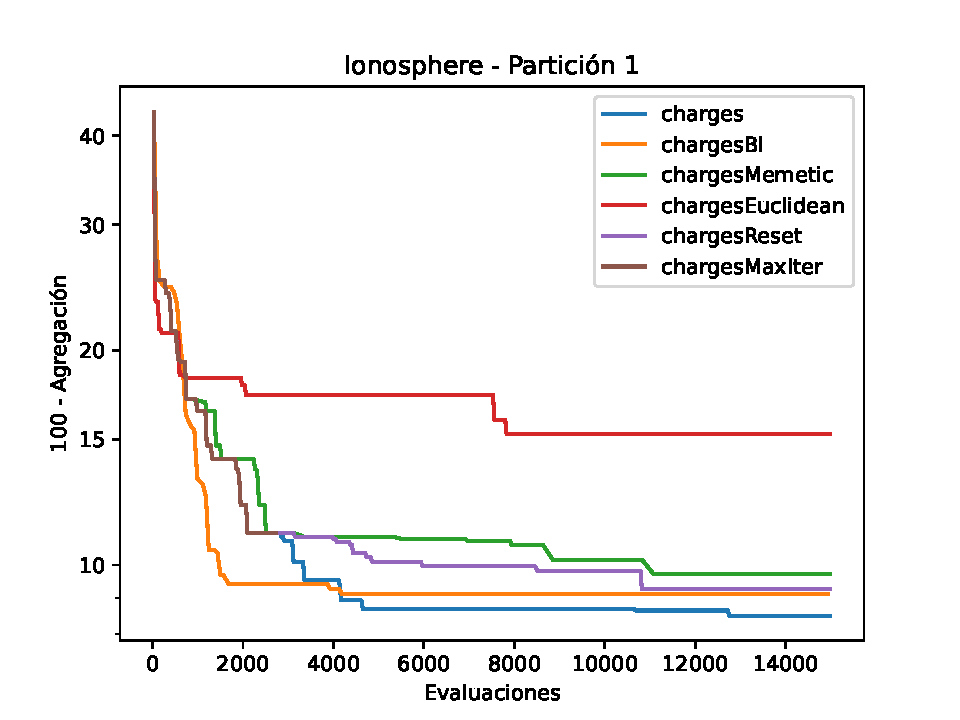
\includegraphics[width=50mm]{../FUENTES/graph/plots/ionosphere1.pdf}}
	\subfigure{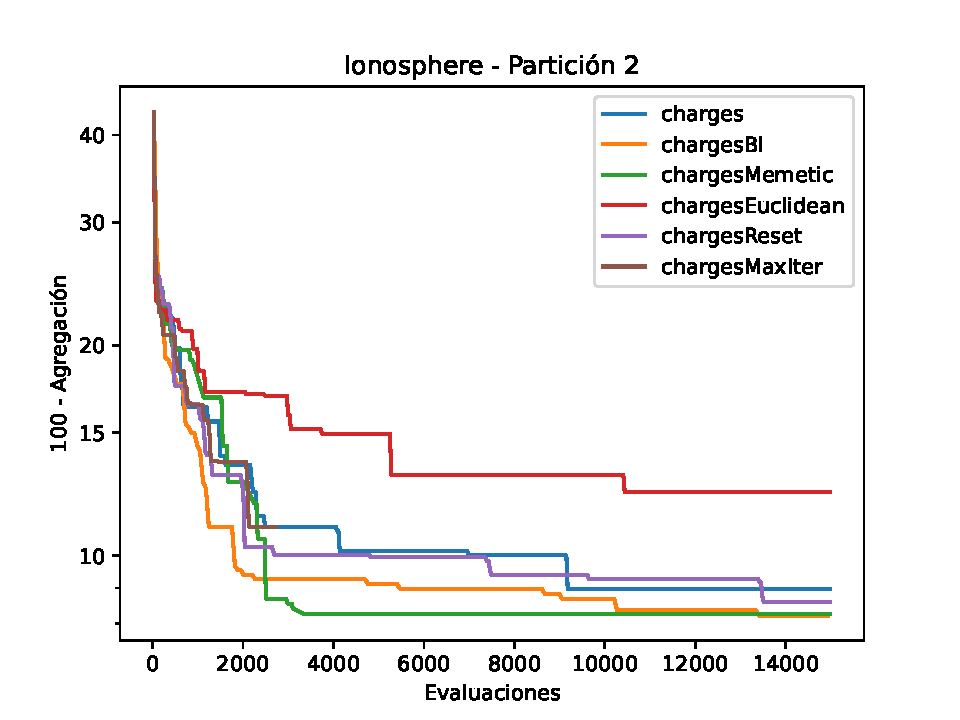
\includegraphics[width=50mm]{../FUENTES/graph/plots/ionosphere2.pdf}}
	\subfigure{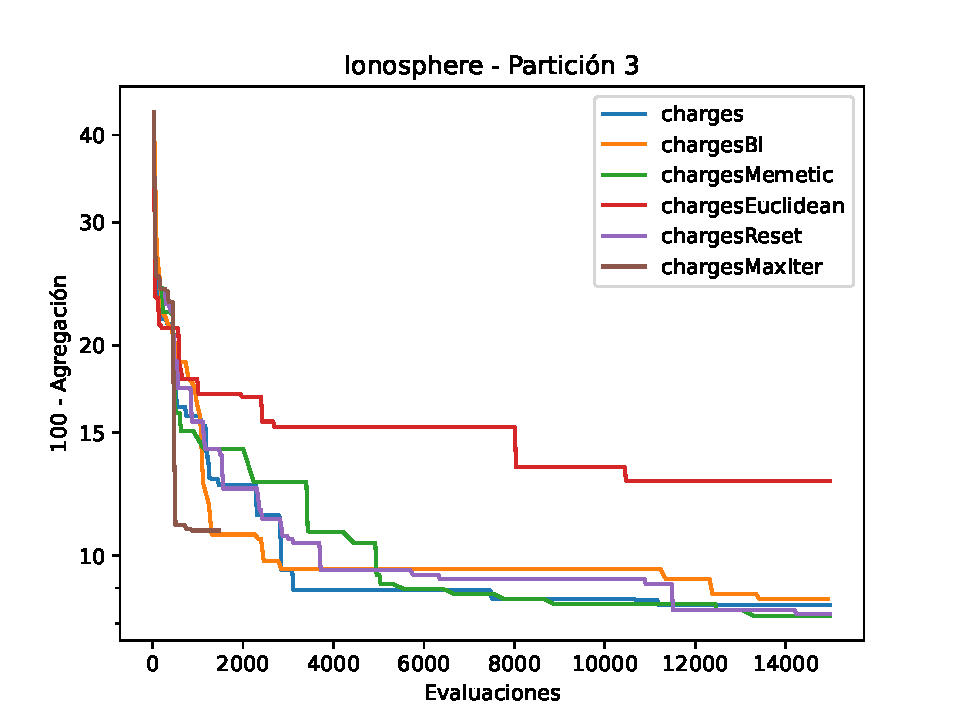
\includegraphics[width=50mm]{../FUENTES/graph/plots/ionosphere3.pdf}}
	\subfigure{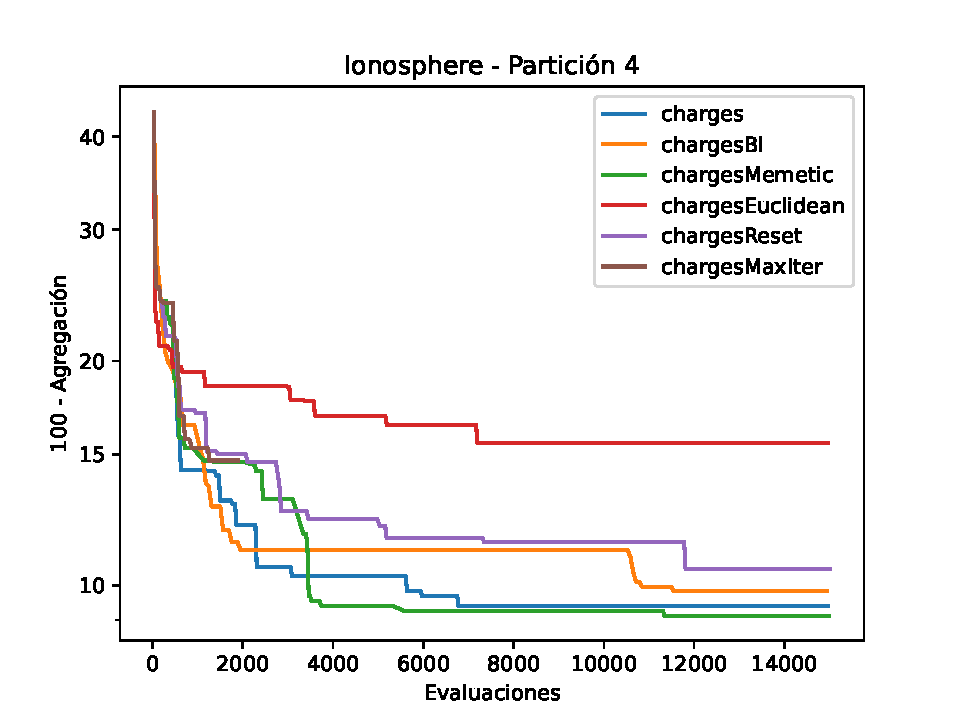
\includegraphics[width=50mm]{../FUENTES/graph/plots/ionosphere4.pdf}}
	\subfigure{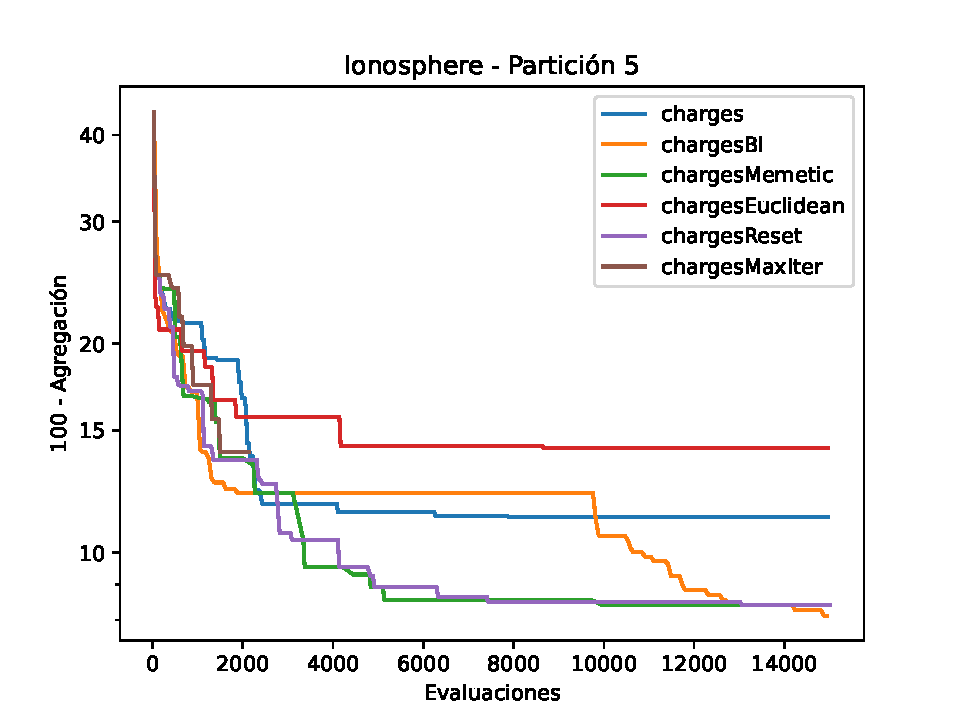
\includegraphics[width=50mm]{../FUENTES/graph/plots/ionosphere5.pdf}}
	\caption{Gráficas de la agregación respecto al número de evaluaciones con los datos de train de Ionosphere}
\end{figure}

\begin{figure}[H]
	\centering
	\subfigure{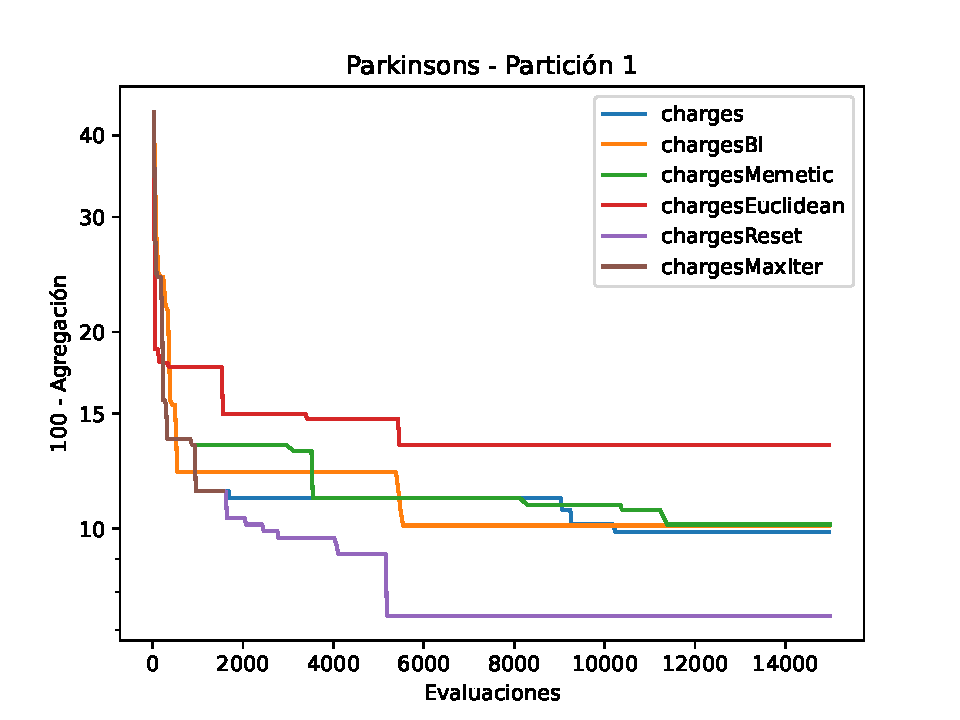
\includegraphics[width=50mm]{../FUENTES/graph/plots/parkinsons1.pdf}}
	\subfigure{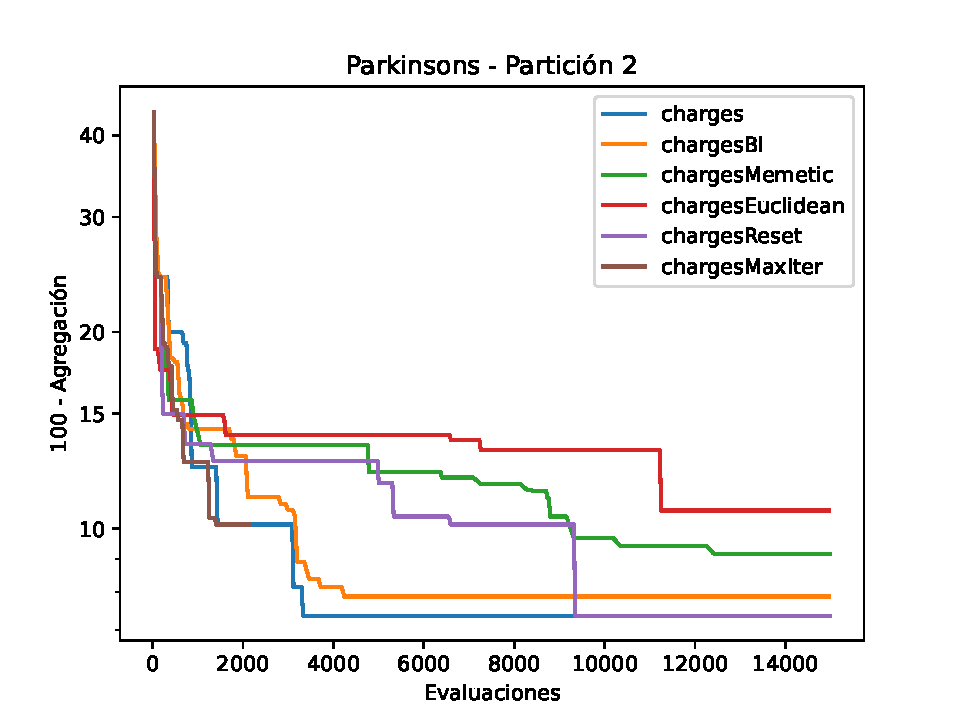
\includegraphics[width=50mm]{../FUENTES/graph/plots/parkinsons2.pdf}}
	\subfigure{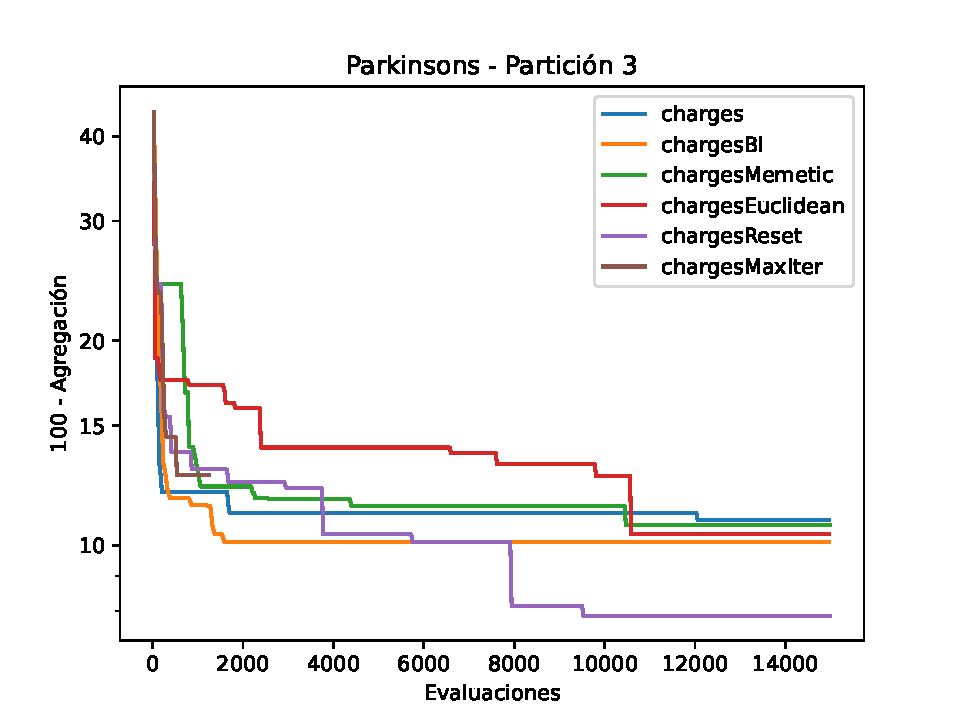
\includegraphics[width=50mm]{../FUENTES/graph/plots/parkinsons3.pdf}}
	\subfigure{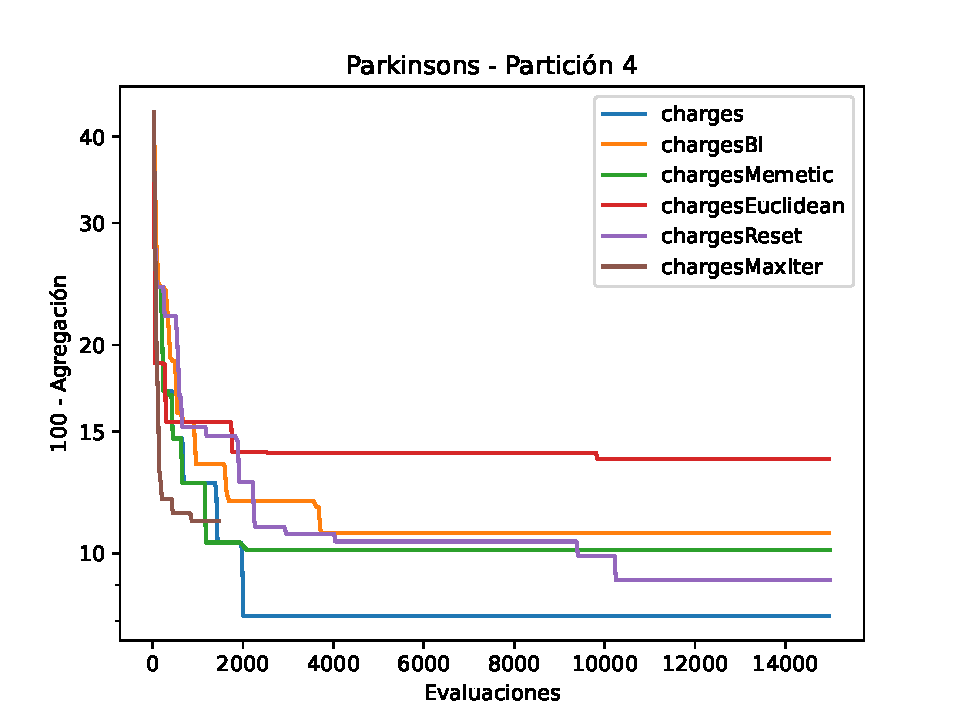
\includegraphics[width=50mm]{../FUENTES/graph/plots/parkinsons4.pdf}}
	\subfigure{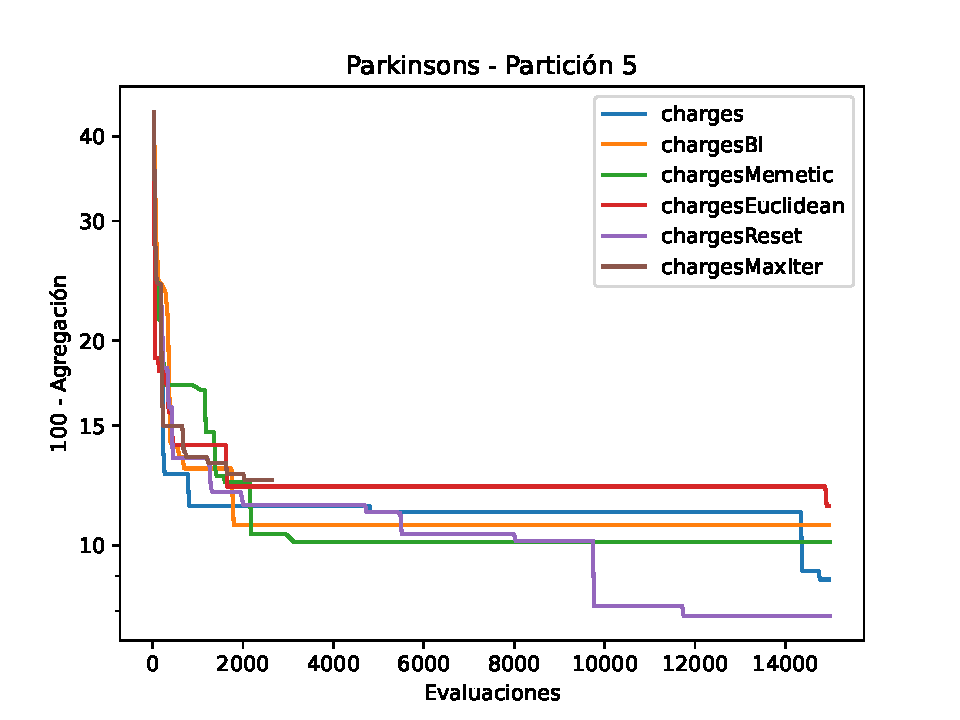
\includegraphics[width=50mm]{../FUENTES/graph/plots/parkinsons5.pdf}}
	\caption{Gráficas de la agregación respecto al número de evaluaciones con los datos de train de Parkinsons}
\end{figure}

\begin{figure}[H]
	\centering
	\subfigure{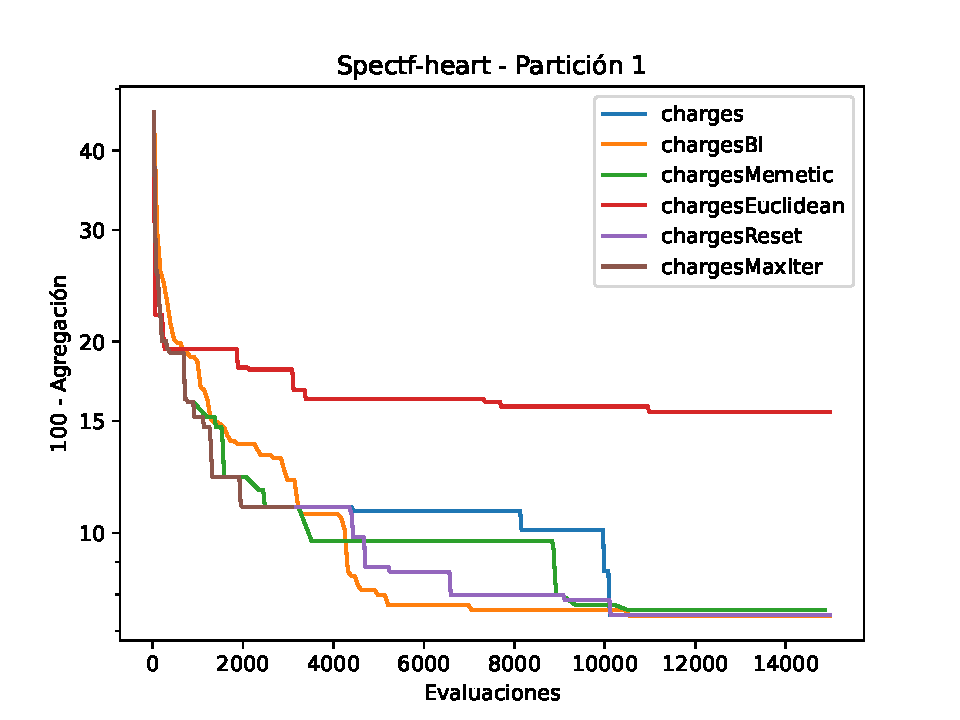
\includegraphics[width=50mm]{../FUENTES/graph/plots/spectf-heart1.pdf}}
	\subfigure{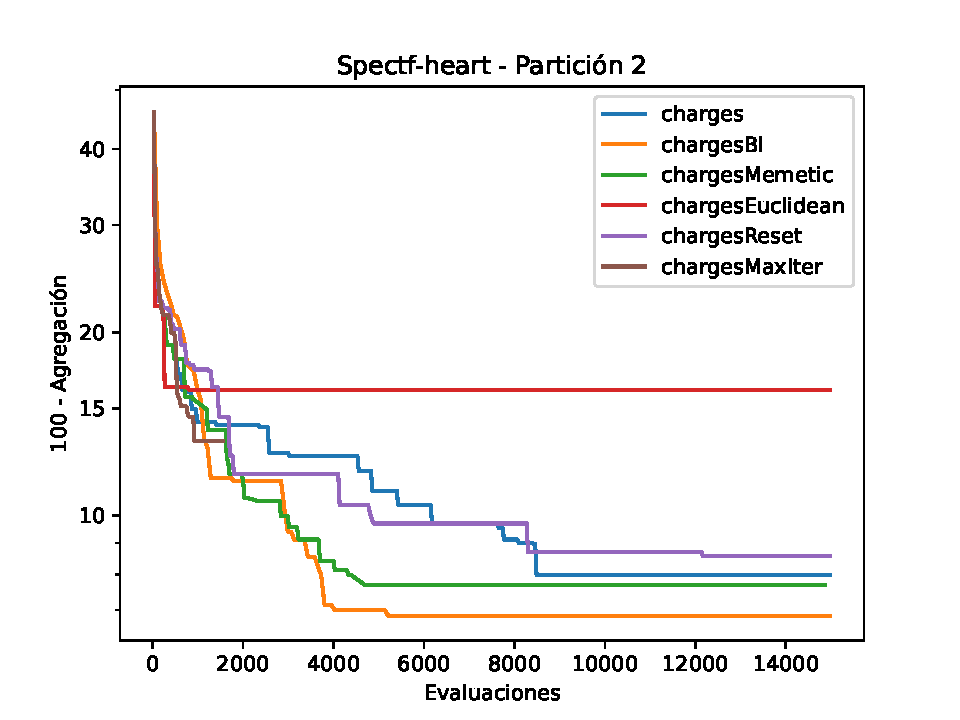
\includegraphics[width=50mm]{../FUENTES/graph/plots/spectf-heart2.pdf}}
	\subfigure{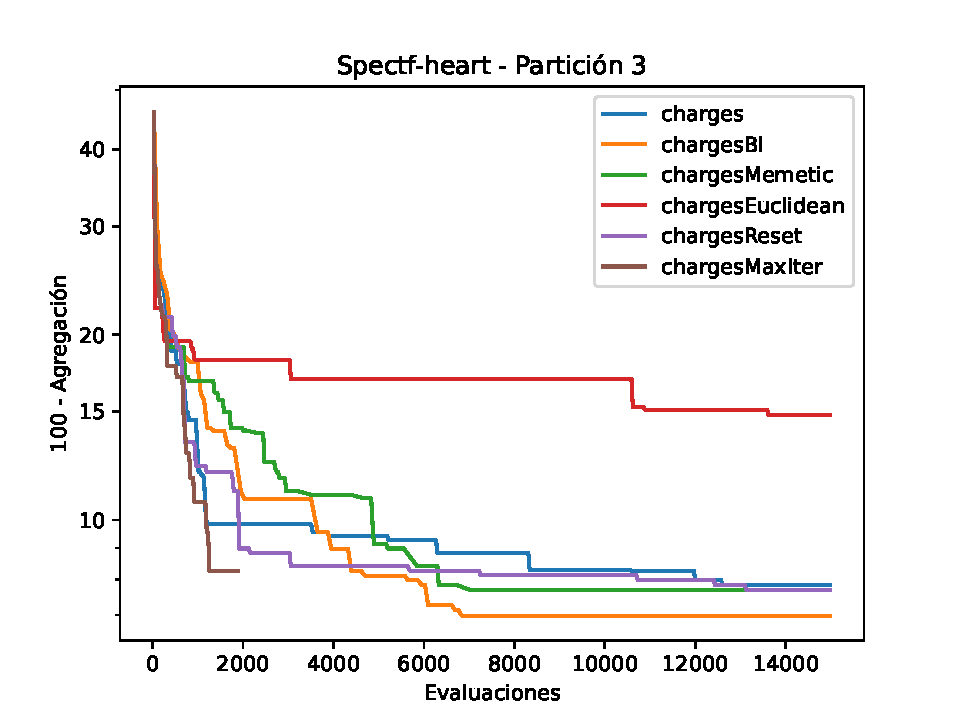
\includegraphics[width=50mm]{../FUENTES/graph/plots/spectf-heart3.pdf}}
	\subfigure{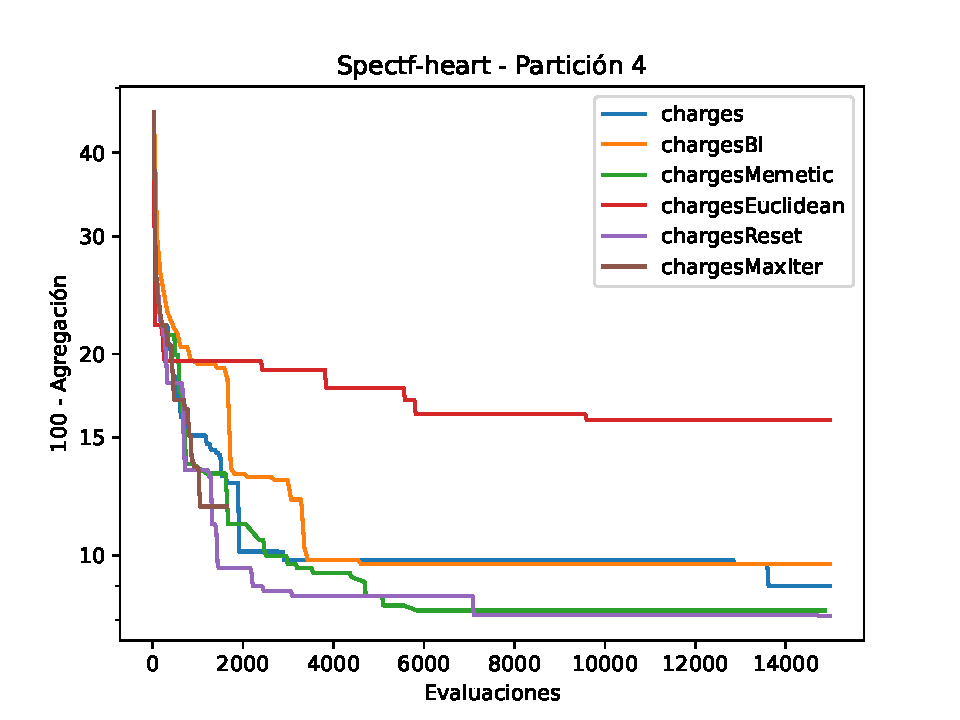
\includegraphics[width=50mm]{../FUENTES/graph/plots/spectf-heart4.pdf}}
	\subfigure{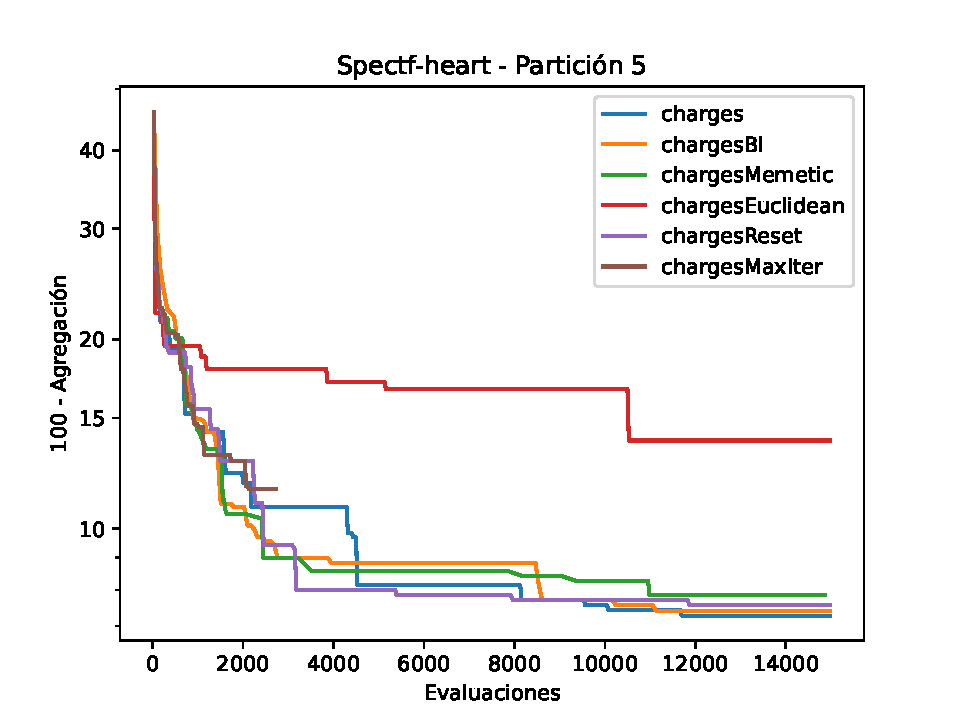
\includegraphics[width=50mm]{../FUENTES/graph/plots/spectf-heart5.pdf}}
	\caption{Gráficas de la agregación respecto al número de evaluaciones con los datos de train de Spectf-heart}
\end{figure}

Nótese que todas estas gráficas muestran la agregación con los datos de entrenamiento, a diferencia de la agregación con los datos de test de la tablas anteriores. Por lo que normalmente estas gráficas mostrarán resultados mejores a los obtenidos en realidad. Sin embargo, si un algoritmo muestra mejores resultados con los datos de entrenamiento, suele significar mejores resultados con los datos de test, aunque no siempre (debido al sobreajuste).

Podemos observar como, en general, \emph{chargesReset} y \emph{chargesMemetic} suelen proporcionar los mejores resultados, aunque en algunas ocasiones son igualados o incluso superados por \emph{charges} y \emph{chargesBl}.

Además, aunque pueda resultar extraño, hay ocasiones en las que \emph{chargesMaxIter} proporciona mejores resultados que \emph{charges}, cuando su funcionamiento es el mismo excepto por el número de evaluaciones. Eso se debe a que, al realizar la comprobación de si la solución mejora o no en cada iteración, modificamos la generación aleatoria, por lo que los resultados pueden ser ligeramente distintos. Sin embargo, al deberse a la aleatoriedad, quiere decir que, de media, si ejecutásemos el algoritmo con infinitas semillas distintas, los resultados serían los mismos.

Por último, podemos observar como \emph{chargesEuclidean} suele proporcionar los peores resultados, lo cuál indica que tomar la distancia en fitness en lugar de la distancia euclídea no sólo supone una mejora en tiempo, si no que también en resultados.

\subsection{Análisis de resultados}

Lo primero que vemos es que \emph{charges} supone una mejora en cuanto a calidad de las soluciones frente a todos los demás algoritmos estudiados en las prácticas anteriores con los datos de \emph{Ionosphere.arff}. Con los datos de \emph{Parkinsons.arff} y \emph{Spectf-heart.arff} también proporciona mejores resultados que la mayoría de algoritmos, siendo superado únicamente por el \emph{enfriamiento simulado} y la \emph{búsqueda local reiterada}.

En cuanto a tiempo de ejecución, es algo más lento que la mayoría de algoritmos, siendo únicamente igualado e, incluso superado, por, de nuevo, el \emph{enfriamiento simulado} y la \emph{búsqueda local reiterada}.

Por lo que tenemos un algoritmo muy potente, superando a todos los estudiados en ciertos casos, aunque es a costa de un elevado tiempo de ejecución.

La versión \emph{chargesMemetic}, que utiliza una hibridación con la búsqueda local, supone una mejora en dos de los tres casos. Además, sólo hemos probado este algoritmo con ciertas combinaciones de número de cromosomas y número de iteraciones entre cada búsqueda local, por lo que es posible encontrar casos en los que los resultados sean aun mayores. Sin embargo, supone un ligero aumento en tiempo, aunque es tan poco que se casi despreciable.

La versión \emph{chargesBl}, que explora el entorno de la mejor solución aplicando búsqueda local a la mejor solución en cada iteración, sólo nos da mejores resultados en un caso, aunque está muy cerca en los otros dos. Debido a esto, es una variante muy potente, y sería interesante si tuviéramos más tiempo probar que tal funciona en otros problemas y con otras semillas, ya que puede llegar a ser una mejoraa.

La versión \emph{chargesEuclidean}, que utiliza la distancia euclídea en lugar de la distancia en fitness, es la que sorprendentemente nos da peores resultados. Debido a que las cargas eléctricas, sistema en el que nos basamos, utilizan la distancia euclídea en el mundo real, cabría esperar una mejora en resultados, o al menos que fueran similares, aunque fuera a costa de un aumento de tiempo. Sin embargo, podemos observar como utilizar la distancia en fitness no sólo disminuye el tiempo de ejecución, si no que mejora los resultados. Aun así, los resultados obtenidos por esta variante siguen superando a muchos de los algoritmos estudiados en las prácticas anteriores, por lo que sigue siendo una buena metaheurística.

La versión \emph{chargesMaxIter}, que se detiene tras un número de iteraciones sin encontrar mejoras, es simplemente una inspiración para \emph{chargesReset}. Aun así, podemos observar como los resultados obtenidos son bastante buenos, y además disminuye mucho el tiempo de ejecución, por lo que, tal y como comentamos durante su explicación, podría ser útil si tratásemos con un sistema en tiempo real, aunque en ese caso también podríamos utilizar la metaheurística original \emph{charges} y detenerla cuando se nos acabe el tiempo.

Por último, tenemos la versión \emph{chargesReset}, que reinicia todas las soluciones menos la mejor a soluciones aleatorias tras varias iteraciones sin encontrar mejora. Aunque es superada en algunos casos por \emph{chargesMemetic}, el \emph{enfriamiento simulado} y la \emph{búsqueda local reiterada}, es el algoritmo que suele dar mejores soluciones, siendo así el más potente estudiado en esta práctica. El hecho de que supere a \emph{charges} en todos los casos nos permite ver la importancia de la exploración del espacio de soluciones. Debido a esto, siempre que el tiempo no sea un factor limitante, es el mejor algoritmo que hemos encontrado.

\newpage
\section{Conclusiones}

\subsection{Valoración de metaheurística}

Tras observar los resultados obtenidos, es interesante ver como lo que en un principio parecía una idea bastante simple ha llegado a superar a la mayoría de los algoritmos estudiados en las prácticas anteriores.

Los mayores inconvenientes que tiene la metaheurística es el tiempo, que es bastante elevado, aunque con ciertas optimizaciones en el código, especialmente a la hora de calcular el fitness de las soluciones, podría solucionarse.

Habría sido interesante haber tenido más tiempo para haber estudiado como se comporta con otros problemas o, al menos, con otras semillas, y para probar a combinar algunas de las modificaciones que hemos realizado.

\subsection{Experiencia diseñando una metaheurística}

Es interesante como, partiendo de una idea tan simple como es que las mejores soluciones atraigan, y las peores repelan, hemos sido capaces de llegar a un algoritmo tan potente.

Los mayores problemas que he tenido durante el desarrollo han sido durante la hibridación con la búsqueda local, ya que tener un número pequeño de cromosomas o aplicar la búsqueda local cada pocas iteraciones proporcionaba peores resultados, por lo que me llevó algún tiempo encontrar una combinación que suponga una mejora, y en pensar posibles mejoras, ya que, aunque la mayoría de ellas parecían prometedoras, proporcionaban peores resultados al implementarlas. Sin embargo, la idea final de \emph{chargesReset} se me ocurrió al ver como se quedaba atascada durante bastantes evaluaciones en las gráficas.

En resumen, estoy muy contento con los resultados, ya que lo que al principio pensaba que era una idea demasiado simple y a la que pensaba que iba a tener que realizar muchas modificaciones o, incluso, modificar por completo por una totalmente nueva, a demostrado ser muy potente, superando a las estudiadas previamente en la asignatura.

\end{document}